\documentclass{article}
\usepackage{pgf}
\usepackage{tikz}
\begin{document}
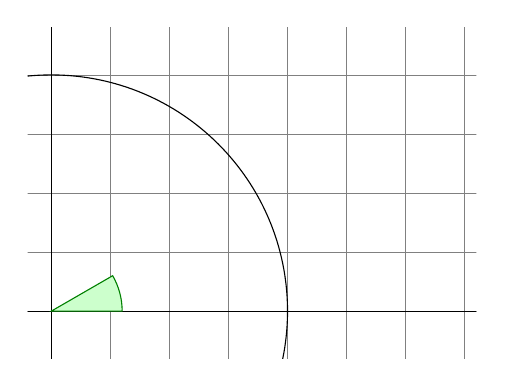
\begin{tikzpicture}[scale=3]
 \clip (-0.1,-0.2)
   rectangle (1.8,1.2);
 \draw[step=.25cm,gray,very thin]
      (-1.4,-1.4) grid (3.4,3.4);
 \draw (-1.5,0) -- (2.5,0);
 \draw (0,-1.5) -- (0,1.5);
 \draw (0,0) circle (1cm);
 \filldraw[fill=green!20!white,
           draw=green!50!black]
	(0,0) -- (3mm,0mm)
             arc (0:30:3mm) -- cycle;
\end{tikzpicture}
\newline
\usetikzlibrary{positioning}
\begin{tikzpicture}[xscale=6,yscale=8,>=stealth]
 \tikzstyle{v}=[circle,
    minimum size=1mm,draw,thick]
 \node[v] (a) {$1$};
 \node[v] (b) [right=of a] {$2$};
 \node[v] (c) [below=of a] {$2$};
 \node[v] (d) [below=of b] {$1$};
 \draw[thick,->]
       (a) to node {} (c);
 \draw[thick,->]
       (a) to node {} (d);
 \draw[thick,->]
       (b) to node {} (d);
\end{tikzpicture}
\end{document}
